\documentclass[11pt,a4j]{jsarticle}
\title{}
\author{1413176 三村幸祐}
\date{2016/12/14}
\usepackage{booktabs}
\usepackage[dvipdfmx,hiresbb]{graphicx}
%\pagestyle{empty}

\begin{document}
  
% \tableofcontents
  
% \newpage
  
  
% 実験の背景と意義、レポートの構成などを記述
 \section{はじめに}
  デジタル信号は0と1の信号の組み合わせでできている。各信号が0と1の2値であるが、現代のデジタル機器では幅広い数値を表現することができる。つまり離散的な値の組み合わせで、見掛け上連続的な幅を表現できるということになる。
  
  ここでは、このコンピュータのシステムを演算装置(ALU)から、Z80コンピュータシステムやI/O制御までを通して理解することを目的とする。
  
  レポートはこの実験全体を2分し、以下のように各レポートで実験結果をまとめる。
  \begin{itemize}
  \item 1部: 演算装置(ALU:Arithmetic Logic Unit)
  \item 2部: Z80コンピュータシステム、I/O制御
  \end{itemize}
  
  そして、このレポートはそのうちの第1部であり、主にデジタル論理回路の演算、またそのオーバフローについて扱う。
  
% 参考書などを用いて、目的と原理を記述
 \section{実験の目的と原理[1]}
  
  \subsection{符号ありと符号なし}
  nビットのデータを扱う場合、それを10進変換するのに2つの方法がある。
   \begin{enumerate}
   \item 符号なし: nビットをそのまま10進変換する方法。正の数のみ扱うことができる。
   \item 符号あり: nビットの表現範囲の約半分を負の表現に使用する方法。最上位ビットが1の場合は負の表現を表す。その場合は-(nビットの2の補数)の絶対値として表現される。
  \end{enumerate}
  
  \subsection{オーバフロー}
  コンピュータは全て2進で行うが、その結果はしばしば10進で計算した解と異なることがある。
  
  たとえば、
  \begin{eqnarray}
  11000000_{(2)} &+& 10110000_{(2)} = 01110000_{(2)} = 112_{(10)} \nonumber \\
  192_{(10)} &+& 176_{(10)} = 368_{(10)} \nonumber
  \end{eqnarray}
  というように、2進での計算結果を10進に直したものと、10進同士で計算した結果が異なる。
  
  このように、コンピュータでの計算が実際の結果と差異を持ってしまうことをオーバフロー、という。
  
  \subsection{シフト演算}
  2進のビットを左右にシフトすることに、論理演算的意義を付加することができる。主に以下のようなプロトコルがある。
  \begin{enumerate}
  \item 論理シフト演算: ビットをひとつづつ左右にずらし、はみ出たビットを捨てて、空いたビットに0を補填する。左シフトは2倍すること、右シフトは2で割ることに相当する。
  \item 算術右シフト演算: ビットをひとつ右にずらし、はみ出したビットを捨てて、空いたビットに元の数の最上位ビットの値を補填する。
  \end{enumerate}
  
  
  
  
% 実験の手順を順次説明
 \section{実験内容}
  
  \begin{enumerate}
  \item Quartus2でHALF\verb|_|ADDER(半加算器),FULL\verb|_|ADDER(全加算器),8bit\verb|_|FULL\verb|_|ADDER(8ビット全加算器),8bit\verb|_|SUBTRACTOR(8ビット減算器)を設計。
  \item 入力Aと入力Bに対する演算出力Oを求めた。ただし7つの全加算器で各ビットごとに計算を行うため、ここでは各入出力についてビットごとに0~7(ex.A0~A7)と表記。
  \item 2の演算結果ごとにオーバフローの有無等について考察。
  \end{enumerate}
  
  
% 図や表による実験データの添付、またそれらの説明を記載
 \section{実験結果}
  
  表\ref{tab:1junbi}にALUの演算入出力応答について事前に予想した準備課題1を示す。
  表\ref{tab:1kadai}には実際のALUの応答結果を示す。準備課題と実験課題の相違点は各表同所に*をもって示す。
  
  これら予想と実際の結果には2と3と4の減算、さらに5で計7箇所の間違えがあったが、これらはすべて
  \begin{itemize}
  \item 計算ミス
  \item 2進から10進変換、及び10進から2進変換時のミス
  \end{itemize}
  にまとめることができる。つまり、人的なミスを除けば予想を外れたような実験結果は生じなかった。
  
  \begin{table}[htb]
  \begin{center}
    \caption{準備課題1}
    \begin{tabular}{|c|c|c|c|c|c|c|c|c|} \hline
課題 & \multicolumn{2}{|c|}{入力A} & \multicolumn{2}{|c|}{入力B} & \multicolumn{2}{|c|}{演算出力} & 桁上がり & 桁借り\\
 & \multicolumn{2}{|c|}{(A7~A0)} & \multicolumn{2}{|c|}{(B7~B0)} & \multicolumn{2}{|c|}{(07~O0)} & (Cout) & (Bout) \\ \cline{2-7}
番号 & 2進表示 & 10進表示 & 2進表示 & 10進表示 & 2進表示 & 10進表示 & キャリー & ボロー \\ \hline
 & 00001010 & 10 & 00001010 &10  &00010100  & 20 & 0 &  \\ \cline{2-8}
1(加) & 01010101 & 85 & 01101010 &106  &10111111  & 191 & 0 & × \\ \cline{2-8}
 & 10000000 & 128 & 01000000 &64  & 11000000 & 192 & 0 &  \\ \hline
 & 00011000 &24  & 00001000 &8  &00010000  & 16 &  & 0 \\ \cline{2-7}\cline{9-9}
1(減) & 01101001 & 105 &00110110  &54  & 00110011 & 51 & × & 0 \\ \cline{2-7}\cline{9-9}
 & 10000000 & 128 &00010000  & 16 &01110000  & 112 &  & 0 \\ \hline
 & 10000001 & 129 &11000000  & 192 &01000001  &65  & 1 &  \\ \cline{2-8}
2(加) & 11000000 & 192 & 01100000 &96  &00100000  &32  & 1 & × \\ \cline{2-8}
 & 10000001 &  129& 10000001 & 129 &00000010  & 2 & 1 &  \\ \hline
 & 00001010 &10  &10100000  &160  &01101010  &106  &  & 1 \\ \cline{2-7}\cline{9-9}
2(減) & 00011110 &  30&01100100*  & 100* & 10111010* &186*  & × & 1 \\ \cline{2-7}\cline{9-9}
 & 10100000 & 160 &11000000  & 192 & 11100000 &224  &  & 1 \\ \hline
 &00001010  & 10 & 00010101 &21  & 00011111 &31  & 0 &  \\ \cline{2-8}
3(加) & 11110000 &-16  & 00110000 & 48 & 00100000 & 32 & 1 & × \\ \cline{2-8}
 & 10110000 & -80 &00011110  & 30 & 11001110 &-50  & 0 &  \\ \hline
 & 01001001 & 73 & 00011100 &28  & 00101101 &45  &  & 0 \\ \cline{2-7}\cline{9-9}
3(減) & 11110000 & -16 &11100000  & -32 &00010000  &16  & × & 0 \\ \cline{2-7}\cline{9-9}
 & 10100000* & 160* & 11000000* & 192* &11100000  &-32  &  & 1 \\ \hline
 &01001001  & 73 &01100100  & 100 & 10101101 & -83 & 0 &  \\ \cline{2-8}
4(加) &  10011000& -104 & 11010001 & -47 & 01101001 &105  & 1 & × \\ \cline{2-8}
 &  10001000&-120  &  10000100& -124 &00001100  & 12 & 1 &  \\ \hline
 &10001000  & -120 & 01000100 & 68 &01000100  & 68 &  & 0 \\ \cline{2-7}\cline{9-9}
4(減) &01010000  & 80 & 10110000 & -80 & 11100000* & -32* & × & 1 \\ \cline{2-7}\cline{9-9}
 &01001001  &73  & 10011100 & -100 &10101101  &-83  &  & 1 \\ \hline
 & 01001010 &74  &00000001  &1  &00100101  & 37 &  &  \\ \cline{2-7}
5(論) &01100000  & 96 & 00000011 & 3 &00001100  &12  & × & × \\ \cline{2-7}
 & 10001010 &-118  & 00000111* &5  & 00000100 &4  &  &  \\ \hline
 &01101001  &105  &00000001  & 1 &00110100  &52  &  &  \\ \cline{2-7}
5(算) & 11100011 & -29 & 00000011 &3  &11111100  &-4  & × & × \\ \cline{2-7}
 & 10001010 & -118 &00000111*  & 5 & 11111100 &-4  &  &  \\ \hline
    \end{tabular}
    \label{tab:1junbi}
  \end{center}
 \end{table}
  
  
  
  
  
  \begin{table}[htb]
  \begin{center}
    \caption{実験課題1(動作検証表)}
    \begin{tabular}{|c|c|c|c|c|c|c|c|c|} \hline
課題 & \multicolumn{2}{|c|}{入力A} & \multicolumn{2}{|c|}{入力B} & \multicolumn{2}{|c|}{演算出力} & 桁上がり & 桁借り\\
 & \multicolumn{2}{|c|}{(A7~A0)} & \multicolumn{2}{|c|}{(B7~B0)} & \multicolumn{2}{|c|}{(07~O0)} & (Cout) & (Bout) \\ \cline{2-7}
番号 & 2進表示 & 10進表示 & 2進表示 & 10進表示 & 2進表示 & 10進表示 & キャリー & ボロー \\ \hline
 & 00001010 & 10 & 00001010 &10  &00010100  & 20 & 0 &  \\ \cline{2-8}
1(加) & 01010101 & 85 & 01101010 &106  &10111111  & 191 & 0 & × \\ \cline{2-8}
 & 10000000 & 128 & 01000000 &64  & 11000000 & 192 & 0 &  \\ \hline
 & 00011000 &24  & 00001000 &8  &00010000  & 16 &  & 0 \\ \cline{2-7}\cline{9-9}
1(減) & 01101001 & 105 &00110110  &54  & 00110011 & 51 & × & 0 \\ \cline{2-7}\cline{9-9}
 & 10000000 & 128 &00010000  & 16 &01110000  & 112 &  & 0 \\ \hline
 & 10000001 & 129 &11000000  & 192 &01000001  &65  & 1 &  \\ \cline{2-8}
2(加) & 11000000 & 192 & 01100000 &96  &00100000  &32  & 1 & × \\ \cline{2-8}
 & 10000001 &  129& 10000001 & 129 &00000010  & 2 & 1 &  \\ \hline
 & 00001010 &10  &10100000  &160  &01101010  &106  &  & 1 \\ \cline{2-7}\cline{9-9}
2(減) & 00011110 &  30& 11000000* & 192* & 01011110* & 94* & × & 1 \\ \cline{2-7}\cline{9-9}
 & 10100000 & 160 &11000000  & 192 & 11100000 &224  &  & 1 \\ \hline
 &00001010  & 10 & 00010101 &21  & 00011111 &31  & 0 &  \\ \cline{2-8}
3(加) & 11110000 &-16  & 00110000 & 48 & 00100000 & 32 & 1 & × \\ \cline{2-8}
 & 10110000 & -80 &00011110  & 30 & 11001110 &-50  & 0 &  \\ \hline
 & 01001001 & 73 & 00011100 &28  & 00101101 &45  &  & 0 \\ \cline{2-7}\cline{9-9}
3(減) & 11110000 & -16 &11100000  & -32 &00010000  &16  & × & 0 \\ \cline{2-7}\cline{9-9}
 & 10100000 & -96* & 11000000 & -64* &11100000  &-32  &  & 1 \\ \hline
 &01001001  & 73 &01100100  & 100 & 10101101 & -83 & 0 &  \\ \cline{2-8}
4(加) &  10011000& -104 & 11010001 & -47 & 01101001 &105  & 1 & × \\ \cline{2-8}
 &  10001000&-120  &  10000100& -124 &00001100  & 12 & 1 &  \\ \hline
 &10001000  & -120 & 01000100 & 68 &01000100  & 68 &  & 0 \\ \cline{2-7}\cline{9-9}
4(減) &01010000  & 80 & 10110000 & -80 & 10100000* & -96* & × & 1 \\ \cline{2-7}\cline{9-9}
 &01001001  &73  & 10011100 & -100 &10101101  &-83  &  & 1 \\ \hline
 & 01001010 &74  &00000001  &1  &00100101  & 37 &  &  \\ \cline{2-7}
5(論) &01100000  & 96 & 00000011 & 3 &00001100  &12  & × & × \\ \cline{2-7}
 & 10001010 &-118  & 00000101* &5  & 00000100 &4  &  &  \\ \hline
 &01101001  &105  &00000001  & 1 &00110100  &52  &  &  \\ \cline{2-7}
5(算) & 11100011 & -29 & 00000011 &3  &11111100  &-4  & × & × \\ \cline{2-7}
 & 10001010 & -118 &00000101*  & 5 & 11111100 &-4  &  &  \\ \hline
    \end{tabular}
    \label{tab:1kadai}
  \end{center}
 \end{table}
 
 
 
 \clearpage
 
 
  
% 実験結果に基づいて課題の回答及びその考察を詳しく記載
 \section{考察}
  以下では、上の実験結果の検証や、それに基づきオーバフロー等に関する考察を行う。
   \subsection{実験結果の検証と解析}
   
   実験結果の検証と解析を行う。内容は付録を参照。
   
   \subsection{各条件におけるオーバフローの法則}
   以下に、符号の有無、加算と減算、に対するオーバフローの発生する法則とその理由を示す。
    \subsubsection{a:符号なしnビット、加算、オーバフローを起こさない法則}
     \begin{itemize}
     \item (条件)10進出力結果が$2^n-1$を越えない2つの数同士の加算。
     \item (理由)最上位ビットからの桁上がりがなく、10進の演算結果が2進の表現可能な範囲に含まれているため。
     \end{itemize}
     
    \subsubsection{b:符号なしnビット、加算、オーバフローを起こす法則}
     \begin{itemize}
     \item (条件)10進出力結果が$2^n$以上となる2つの数同士の加算。
     \item (理由)10進の演算結果が2進の表現可能な範囲に含まれていないため。
     \end{itemize}
     
    \subsubsection{c:符号なしnビット、減算、オーバフローを起こさない法則}
    \begin{itemize}
     \item (条件)「引かれる数A」より「引く数B」の方が小さい。
     \item (理由)10進出力が引かれる数より小さい正の数になり、2進nビットで表現可能であるため。
     \end{itemize}
    
    \subsubsection{d:符号なしnビット、減算、オーバフローを起こす法則}
    \begin{itemize}
     \item (条件)「引かれる数A」より「引く数B」の方が大きい。
     \item (理由)10進出力が負の数になり、符号なし2進で表現で着ないため。
     \end{itemize}
    
    \subsubsection{e:符号ありnビット、加算、オーバフローを起こさない法則}
    \begin{itemize}
     \item (条件)1.異符号同士の加算。2.10進出力結果の絶対値が$2^n-1$を越えない同符号同士の加算。
     \item (理由)1.10進出力結果の絶対値が$2^n-1$を越えず、符号ビットを除く部分(n-1ビット)で表現で切るため。2.符号ビットを除くn-1ビットで$2^{n-1}-1$までの絶対値を表現できるため。
     \end{itemize}
    
    \subsubsection{f:符号ありnビット、加算、オーバフローを起こす法則}
    \begin{itemize}
     \item (条件)10進出力結果の絶対値が'$2^n$以上となる同符号同士の加算。
     \item (理由)最上位ビットを除くn-1ビット数では$2^n-1$を越える絶対値を表現できないため。
     \end{itemize}
    
    \subsubsection{g:符号ありnビット、減算、オーバフローを起こさない法則}
    \begin{itemize}
     \item (条件)1.同符号同士の減算。2.10進出力の絶対値が$2^{n-1}-1$を越えない異符号間の減算。
     \item (理由)1.10進出力結果の絶対値が$2^{n-1}-1$を越えず、符号ビットを除く部分(n-1ビット)で表現で切るため。2.符号ビットを除くn-1ビット数で$2^{n-1}-1$までの絶対値を表現できるため。
     \end{itemize}
    
    \subsubsection{h:符号ありnビット、減算、オーバフローを起こす法則}
    \begin{itemize}
     \item (条件)10進出力結果の絶対値が$2^{n-1}$以上となる異符号間の減算。
     \item (理由)最上位ビットを除くn01ビットでは$2^{n-1}-1$を越える絶対値を表現できないため。
     \end{itemize}
    
   
   
   
   \subsection{オーバフローの検出真理値表、論理式及びその回路}
   以下に、符号の有無、加算と減算、に対するオーバフローを検出する真理値表と論理式、及びその回路を示す。
    \subsubsection{a:符号なし、加算}
    
    \begin{itemize}
    \item (真理値表)
    
    \begin{table}[htb]
  \begin{center}
    \caption{符号なし、加算、のオーバフロー真理値表}
    \begin{tabular}{cccc|c} \toprule
ADDSUB & SIGN & COUT & BOUT & overflow \\ \midrule
0 & 0 & 0 & 0 & 0(無) \\
0 & 0 & 1 & 0 & 1(有) \\ \bottomrule
    \end{tabular}
    \label{}
  \end{center}
 \end{table}
    
    \item (論理式)
    
    \begin{equation}
    overflow = COUT
    \end{equation}
    
    \item (回路図)
    
    \begin{figure}[htbp]
  \centering
  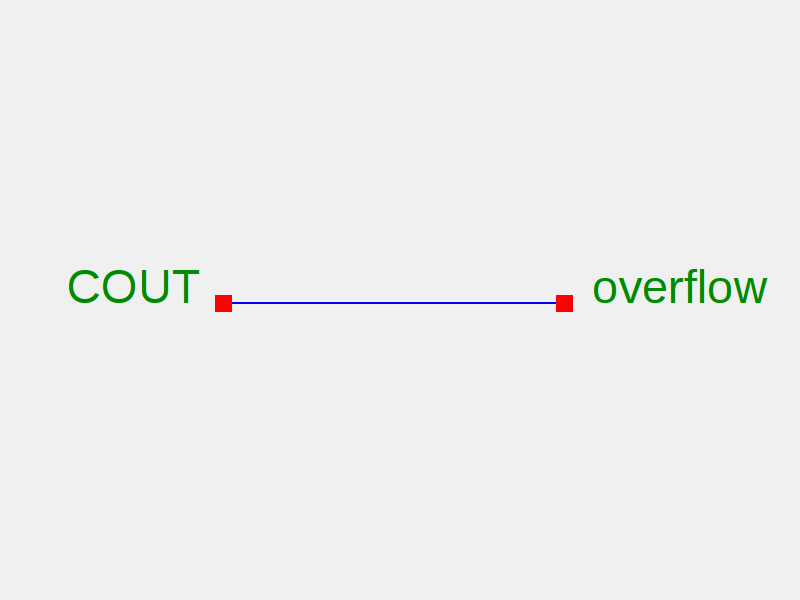
\includegraphics[width=4cm,clip]{3-a.png}
  \caption{符号なし、加算、のオーバフロー検出回路}
  \label{fig:3-a}
 \end{figure}
    
    
    \end{itemize}
    
    
    
    \subsubsection{b:符号なし、減算}
    
    \begin{itemize}
    
    \item (真理値表)
    8ビットALU、加減算、オーバフロー
    \begin{table}[htb]
  \begin{center}
    \caption{符号なし、減算、オーバフロー真理値表}
    \begin{tabular}{cccc|c} \toprule
ADDSUB & SIGN & COUT & BOUT & overflow \\ \midrule
1 & 0 & 0 & 0 & 0 \\
1 & 0 & 0 & 1 & 1 \\ \bottomrule
    \end{tabular}
    \label{}
  \end{center}
 \end{table}
    
    \item (論理式)
    
    \begin{equation}
    overflow = BOUT
    \end{equation}
    
    \item (回路図)
    
    \begin{figure}[htbp]
  \centering
  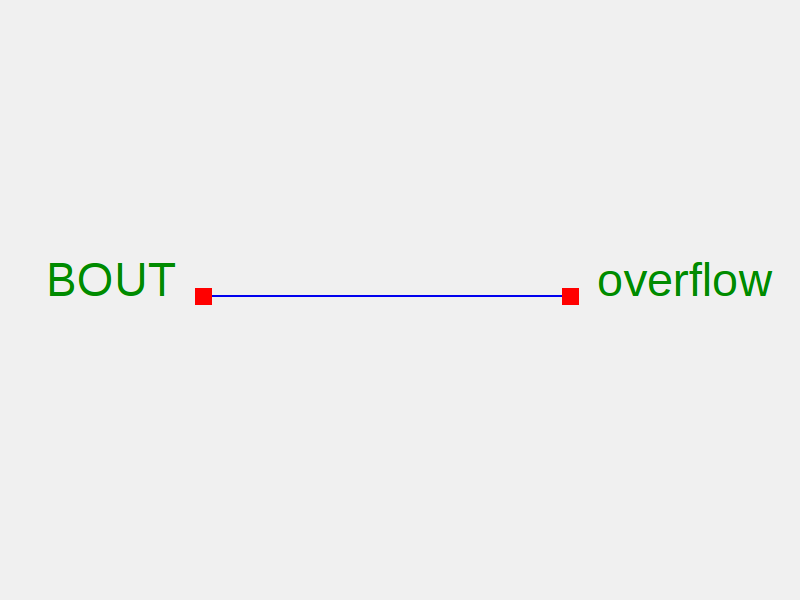
\includegraphics[width=4cm,clip]{3-b.png}
  \caption{符号なし、減算、オーバフロー検出回路}
  \label{fig:3-b}
 \end{figure}
    
    \end{itemize}
    
    \clearpage
    
    \subsubsection{c:符号あり、加算}
    
    \begin{itemize}
    
    \item (真理値表)
    
    \begin{table}[htb]
  \begin{center}
    \caption{符号あり、加算、オーバフロー真理値表}
    \begin{tabular}{ccccc|c} \toprule
ADDSUB & SIGN & A7 & B7 & O7 & overflow \\ \midrule
0 & 1 & 0 & 0 & 0 & 0 \\
0 & 1 & 0 & 0 & 1 & 1 \\
0 & 1 & 1 & 1 & 1 & 0 \\
0 & 1 & 1 & 1 & 0 & 1 \\
0 & 1 & 0 & 1 & 0 & 0 \\
0 & 1 & 1 & 0 & 0 & 0 \\ \bottomrule
    \end{tabular}
    \label{}
  \end{center}
 \end{table}
    
    \item (論理式)
    
    \begin{equation}
    overflow = (\overline{A7 \bigoplus B7}) \bigwedge (A7 \bigoplus O7)
    \end{equation}
    
    \item (回路図)
    
    \begin{figure}[htbp]
  \centering
  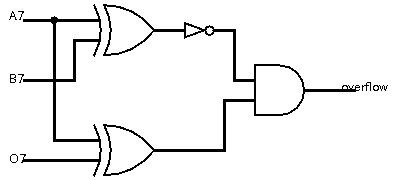
\includegraphics[width=8cm,clip]{3-c.png}
  \caption{符号あり、加算、オーバフロー検出回路}
  \label{fig:3-c}
 \end{figure}
    
    \end{itemize}
    
    \clearpage
    
    \subsubsection{d:符号あり、減算}
    
    \begin{itemize}
    
    \item (真理値表)
    
     \begin{table}[htb]
  \begin{center}
    \caption{符号あり、減算、オーバフロー真理値表}
    \begin{tabular}{ccccc|c} \toprule
ADDSUB & SIGN & A7 & B7 & O7 & overflow \\ \midrule
1 & 1 & 0 & 0 & 0 & 0 \\
1 & 1 & 0 & 0 & 1 & 0 \\
1 & 1 & 1 & 1 & 0 & 0 \\
1 & 1 & 1 & 1 & 1 & 0 \\
1 & 1 & 0 & 1 & 0 & 0 \\
1 & 1 & 0 & 1 & 1 & 1 \\
1 & 1 & 1 & 0 & 1 & 0 \\
1 & 1 & 1 & 0 & 0 & 1 \\ \bottomrule
    \end{tabular}
    \label{}
  \end{center}
 \end{table}
    
    \item (論理式)
    
    \begin{equation}
    overflow = (A7 \bigoplus B7) \bigwedge (A7 \bigoplus O7)
    \end{equation}
    
    \item (回路図)
    
    \begin{figure}[htbp]
  \centering
  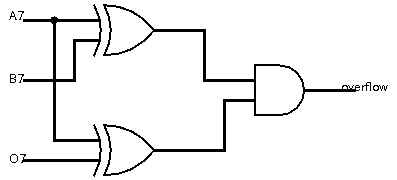
\includegraphics[width=8cm,clip]{3-d.png}
  \caption{符号あり、減算、オーバフロー検出回路}
  \label{fig:3-d}
 \end{figure}
    
    \end{itemize}
    
    \clearpage
    
    \subsubsection{e:8ビットALU、加減算}
    
    \begin{itemize}
    
    \item (真理値表)
    
     \begin{table}[htb]
  \begin{center}
    \caption{8ビットALU、加減算、オーバフロー真理値表}
    \begin{tabular}{cc|ccc|cc|c} \toprule
ADDSUB & SIGN & A7 & B7 & O7 & COUT & BOUT & overflow \\ \midrule
0 & 0 &  &  &  & 0 & 0 & 0(無) \\
0 & 0 &  &  &  & 1 & 0 & 1(有) \\ \midrule
1 & 0 &  &  &  & 0 & 0 & 0 \\
1 & 0 &  &  &  & 0 & 1 & 1 \\ \midrule
0 & 1 & 0 & 0 & 0 &  &  & 0 \\
0 & 1 & 0 & 0 & 1 &  &  & 1 \\
0 & 1 & 1 & 1 & 1 &  &  & 0 \\
0 & 1 & 1 & 1 & 0 &  &  & 1 \\
0 & 1 & 0 & 1 & 0 &  &  & 0 \\
0 & 1 & 1 & 0 & 0 &  &  & 0 \\ \midrule
1 & 1 & 0 & 0 & 0 &  &  & 0 \\
1 & 1 & 0 & 0 & 1 &  &  & 0 \\
1 & 1 & 1 & 1 & 0 &  &  & 0 \\
1 & 1 & 1 & 1 & 1 &  &  & 0 \\
1 & 1 & 0 & 1 & 0 &  &  & 0 \\
1 & 1 & 0 & 1 & 1 &  &  & 1 \\
1 & 1 & 1 & 0 & 1 &  &  & 0 \\
1 & 1 & 1 & 0 & 0 &  &  & 1 \\ \bottomrule
    \end{tabular}
    \label{}
  \end{center}
 \end{table}
    
    \item (論理式)
    
    \begin{eqnarray}
    overflw &=& \overline{SIGN} \bigwedge (COUT \bigvee BOUT) \nonumber \\
                  && \bigvee SIGN \bigwedge \overline{ADDSUB} \bigwedge (\overline{A7 \bigoplus B7}) \bigwedge (A7 \bigoplus O7) \nonumber \\
                  && \bigvee SIGN \bigwedge ADDSUB \bigwedge (A7 \bigoplus B7) \bigwedge (A7 \bigoplus O7)
    \end{eqnarray}
    
    \item (回路図)
    
    \begin{figure}[htbp]
  \centering
  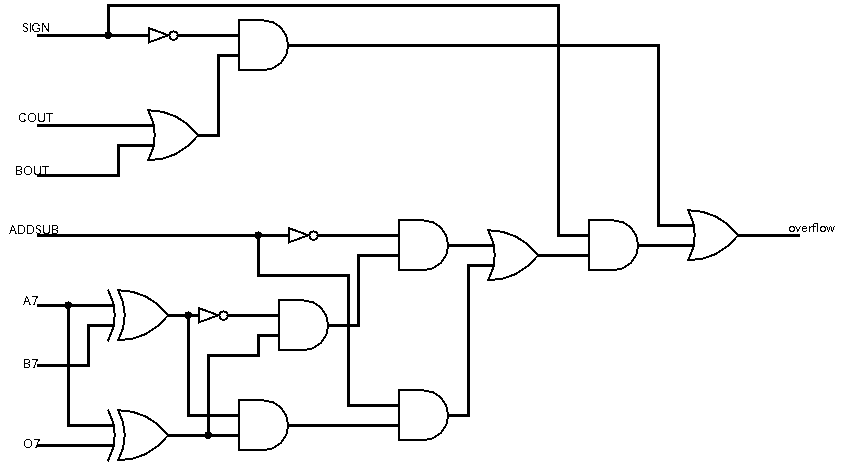
\includegraphics[width=8cm,clip]{3-e.png}
  \caption{8ビットALU、加減算、オーバフロー検出回路}
  \label{fig:3-e}
 \end{figure}
    
    
    \end{itemize}
    
    
   
   
  
  
% まとめ
 \section{おわりに}
  
  今回の実験では、デジタル演算器での論理演算についてその方法とオーバフローについて主に検証した。
  するとデジタル演算は予測に沿った能力を持ち合わせながらも多くの例外によるオーバフローの発生も多発することがわかる。しかしそのオーバフローもある法則によって検出、制御することまで今回学んだため、計算内容によって演算プロトコルを制御すればデジタル演算には高い正確性を持たせることができる、という結果になった。
  
  
% 参考文献の列挙
 \section{参考文献}
  [1]雨宮好文,「現代電子回路学[2]」,オーム社,p.131~146
  
  
\end{document}